%versi 2 (8-10-2016)
\chapter{Analisis dan Perancangan}
\label{chap:analisisdanperancangan}
Bab ini membahas analisis domain masalah, spesifikasi kebutuhan, diagram yang digunakan untuk perancangan dan perancangan situs. Rancangan dasar proyek ini akan mengikuti bentuk dari bagian penerbangan dan hotel untuk konsistensi tampilan.

\section{Analisis Domain Masalah}
\label{sec:analisisdomainmasalah} 

Sesuai latar belakang yang diberikan di \ref{sec:latarbelakang}, sebuah perusahaan \textit{tour and travel} meminta sebuah situs web yang mirip dengan yang sudah dibuat sebelumnya dengan tambahan pemesanan tiket kereta api. Untuk memenuhi kebutuhan ini, diperlukan pengumpulan data dari berbagai situs pemesanan tiket kereta api lain. Dari hasil pembandingan yang dilakukan dari beberapa situs pemesanan tiket yang ada, dapat diambil kesimpulan bahwa modul ini membutuhkan:

\begin{table}[H]
	\centering 
	\caption{Tabel Kebutuhan Modul Kereta Api}
	\label{tab:kebutuhankeretaapi}
	\begin{tabular}{|p{5cm}|p{5cm}|}
		\hline
		Kebutuhan & Solusi\\
		\hline
		
		\hline
		Tempat pengguna bisa memberikan parameter pencarian tiket & Halaman untuk memasukkan \textit{input} dan mencari tiket\\
		\hline
		Tempat pengguna bisa memilih jadwal tiket & Halaman untuk menampilkan dan memilih jadwal kereta\\
		\hline
		Tempat pengguna bisa mengisi data pemesan dan penumpang & Halaman untuk mengisi data pemesan dan penumpang\\
		\hline
		Tempat pengguna bisa memilih tempat duduk & Halaman untuk menampilkan bentuk pemetaan kursi kereta dan memilih kursi\\
		\hline
		Tempat pengguna bisa melihat informasi transaksi & Halaman untuk menampilkan informasi-informasi pemesanan\\
		\hline
		Tempat pengguna bisa membayar pemesanan & Halaman untuk melakukan pembayaran\\
		\hline
		
	\end{tabular} 
\end{table}

Untuk menambah modul pembuatan kereta api, sistem yang sudah ada sebelumnya perlu dipelajari terlebih dahulu. Dengan membandingkan beberapa situs pemesanan tiket kereta api lain dengan sistem yang sudah ada, dapat disimpulkan bahwa beberapa kebutuhan yang tertera di tabel \ref{tab:kebutuhankeretaapi} memiliki kemiripan dengan pemesanan tiket penerbangan. Bagian penerbangan sudah memiliki halaman pencarian tiket, halaman penampilan jadwal, halaman pengisian data dan halaman konfirmasi dengan halaman eksternal pembayaran menggunakan \textit{API}. Penyesuaian dan perancangan yang dibuat dengan menggabungkan hasil pembelajaran ini dapat dilihat pada \ref{sec:perancanganhalaman}.

\section{Diagram Use Case}
\label{sec:usecase} 

Sistem pemesanan tiket kereta api yang dibangun dapat membantu pengguna memesan tiket kereta api secara \textit{online}. Fitur-fitur yang dapat dilakukan sistem dapat digambarkan dengan diagram \textit{use case} seperti pada gambar \ref{img:usecasediagram}. Diagram \textit{use case} yang ditampilkan di sini hanya membahas kasus-kasus yang berhubungan langsung dengan sistem yang dibangun. \textit{Use case} untuk admin tidak dibawa di sini karena itu merupakan fitur bawaan dari sistem keseluruhan. 

\begin{figure}[H]
\center
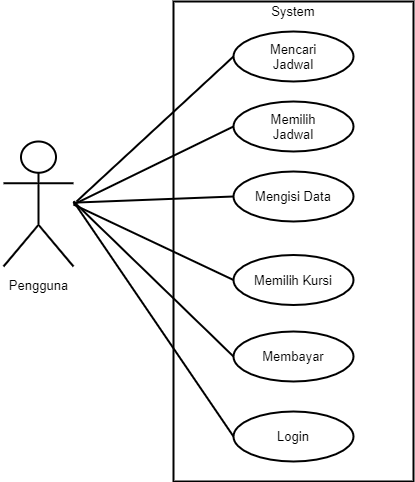
\includegraphics[scale=0.8]{Gambar/Use Case Diagram.png}
\caption{\textit{Use Case Diagram.}}
    \label{img:usecasediagram}
\end{figure}

Melihat dari diagram tersebut, dapat dibuat skenario untuk masing-masing \textit{use case} sebagai berikut:

\begin{itemize}
    \item Mencari Jadwal
	
	\textbf{Name: }Mencari Jadwal\\
	\textbf{Actors: }Pengguna (orang yang ingin memesan tiket)\\
	\textbf{Goals: }Pengguna bisa memasukkan \textit{input} pencarian\\
	\textbf{Precondition: }Pengguna sudah membuka situs perusahaan \textit{client}\\
	\textbf{Steps: }
	\begin{table}[H]
		\centering
		\caption{Skenario use case "Mencari Jadwal"}
		\label{tab:usecase1} 
		\begin{tabular}{|p{7cm}|p{7cm}|}
			\hline
			\textbf{Actor actions} & \textbf{System responses} \\ \hline
			1. Pengguna masuk ke halaman pencarian tiket kereta api & \\
			  & 2. Halaman pencarian jadwal ditampilkan \\
			3. Pengguna memasukkan data berupa perjalanan satu arah atau pulang pergi, stasiun awal dan tujuan, tanggal keberangkatan dan tanggal pulang (opsional), jumlah penumpang &\\ 
			4. Pengguna menekan tombol "cari" & \\
			  & 5. Sistem meneruskan parameter pencarian dan mengarahkan pengguna ke halaman pemilihan jadwal\\
			\hline
		\end{tabular}
	\end{table}	
	
	\item Memilih Jadwal
	
	\textbf{Name: }Memilih Jadwal\\
	\textbf{Actors: }Pengguna (orang yang ingin memesan tiket)\\
	\textbf{Goals: }Pengguna bisa memilih jadwal kereta yang diinginkan\\
	\textbf{Precondition: }Pengguna sudah masuk ke halaman memilih jadwal\\
	\textbf{Steps: }
	\begin{table}[H]
		\centering
		\caption{Skenario use case "Mencari Jadwal"}
		\label{tab:usecase2} 
		\begin{tabular}{|p{7cm}|p{7cm}|}
			\hline
			\textbf{Actor actions} & \textbf{System responses} \\ \hline
			1. Pengguna masuk ke halaman pemilihan jadwal kereta api & \\
			  & 2. Halaman menampilkan jadwal sesuai dengan \textit{input} pengguna \\
			3. Pengguna memilih jadwal kereta yang pengguna inginkan &\\ 
			4. Pengguna menekan tombol "selanjutnya" & \\
			  & 5. Sistem mencatat jadwal yang sudah dipilih pengguna dan mengarahkan pengguna ke halaman pengisian data\\
			\hline
		\end{tabular}
	\end{table}	
	
	\item Mengisi Data
	
	\textbf{Name: }Mencari Jadwal\\
	\textbf{Actors: }Pengguna (orang yang ingin memesan tiket)\\
	\textbf{Goals: }Pengguna bisa memasukkan data pemesan dan penumpang\\
	\textbf{Precondition: }Pengguna sudah memilih jadwal dan masuk ke halaman pengisian data\\
	\textbf{Steps: }
	\begin{table}[H]
		\centering
		\caption{Skenario use case "Mengisi Data"}
		\label{tab:usecase3} 
		\begin{tabular}{|p{7cm}|p{7cm}|}
			\hline
			\textbf{Actor actions} & \textbf{System responses} \\ \hline
			1. Pengguna masuk ke halaman pengisian data & \\
			  & 2. Halaman pengisian data menampilkan \textit{form} yang harus diisi pengguna \\
			3. Pengguna memasukkan data berupa \textit{title}, nama, email dan nomor telepon ke data pemesan & \\ 
			4. Pengguna memasukkan data berupa nama dan identitas ke data penumpang & \\
			5. Pengguna menekan "pilih kursi" atau "selanjutnya" & \\
			  & 6. Sistem meneruskan data pemesan dan penumpang kemudian mengarahkan pengguna ke halaman sesuai dengan pilihan pengguna (pilih kursi mengarah ke halaman pilih kursi, selanjutnya mengarah ke pembayaran)\\
			\hline
		\end{tabular}
	\end{table}	
	
	\item Memilih Kursi
	
	\textbf{Name: }Memilih Kursi\\
	\textbf{Actors: }Pengguna (orang yang ingin memesan tiket)\\
	\textbf{Goals: }Pengguna bisa memilih kursi baru\\
	\textbf{Precondition: }Pengguna sudah masuk ke halaman pemilihan kursi\\
	\textbf{Steps: }
	\begin{table}[H]
		\centering
		\caption{Skenario use case "Memilih Kursi"}
		\label{tab:usecase4} 
		\begin{tabular}{|p{7cm}|p{7cm}|}
			\hline
			\textbf{Actor actions} & \textbf{System responses} \\ \hline
			1. Pengguna masuk ke halaman pemilihan kursi & \\
			  & 2. Halaman pemilihan kursi menampilkan data penumpang dan peta pemilihan kursi \\
			3. Pengguna memilih kursi yang diinginkan sejumlah penumpang dewasa dengan menekan kursi yang diinginkan di peta &\\ 
			  & 4. Sistem mengubah warna kursi sehingga pengguna tahu kursi sudah berubah\\
			5. Pengguna menekan tombol "selanjutnya" & \\
			  & 6. Sistem meneruskan data perubahan kursi dan mengarahkan pengguna ke halaman pembayaran\\
			\hline
		\end{tabular}
	\end{table}	
	
	\item Membayar
	
	\textbf{Name: }Membayar\\
	\textbf{Actors: }Pengguna (orang yang ingin memesan tiket)\\
	\textbf{Goals: }Pengguna bisa melakukan pembayaran\\
	\textbf{Precondition: }Pengguna sudah masuk halaman pembayaran\\
	\textbf{Steps: }
	\begin{table}[H]
		\centering
		\caption{Skenario use case "Membayar"}
		\label{tab:usecase5} 
		\begin{tabular}{|p{7cm}|p{7cm}|}
			\hline
			\textbf{Actor actions} & \textbf{System responses} \\ \hline
			1. Pengguna masuk ke halaman pembayaran & \\
			  & 2. Halaman pembayaran menampilkan detail transaksi pengguna \\
			3. Pengguna menekan tombol bayar & \\
			  & 4. Sistem mengarahkan pengguna ke halaman pembayaran eksternal\\
			5. Pengguna melakukan pembayaran & \\
			  & 6. Sistem menerima notifikasi pembayaran dan mengarahkan pengguna kembali ke halawan utama\\
			\hline
		\end{tabular}
	\end{table}	
	
	\item \textit{Login}
	
	\textbf{Name: }\textit{Login}\\
	\textbf{Actors: }Pengguna (orang yang ingin memesan tiket)\\
	\textbf{Goals: }Pengguna bisa masuk ke akun miliknya yang sudah terdaftar\\
	\textbf{Precondition: }Pengguna sudah memiliki akun yang terdaftar\\
	\textbf{Steps: }
	\begin{table}[H]
		\centering
		\caption{Skenario use case "\textit{Login}"}
		\label{tab:usecase6} 
		\begin{tabular}{|p{7cm}|p{7cm}|}
			\hline
			\textbf{Actor actions} & \textbf{System responses} \\ \hline
			1. Pengguna masuk ke halaman \textit{login} & \\
			  & 2. Halaman menampilkan \textit{form} untuk \textit{login} berupa email dan kata sandi \\
			3. Pengguna memasukkan email dan kata sandi & \\ 
			4. Pengguna menekan tombol "\textit{login}" & \\
			  & 5. Sistem memeriksa apakah data yang dimasukkan benar\\
			  & 6a. Jika benar pengguna akan berhasil \textit{login} dan dikembalikan ke halaman sebelum pengguna masuk ke halaman \textit{login}\\
			  & 6b. Jika salah, pengguna mengulang dari langkah ke-3\\
			\hline
		\end{tabular}
	\end{table}	
	
	
\end{itemize}

\section{Diagram Kelas}
\label{sec:diagramkelas}

Pada subbab ini akan dibahas diagram kelas yang digunakan dalam pembangunan proyek ini. Diagram kelas yang ditampilkan di sini hanyalah mencakup kelas-kelas yang digunakan dalam pembangunan proyek ini. Diagram kelas dapat dilihat pada gambar \ref{img:classdiagram}.

\begin{figure}[H]
\center
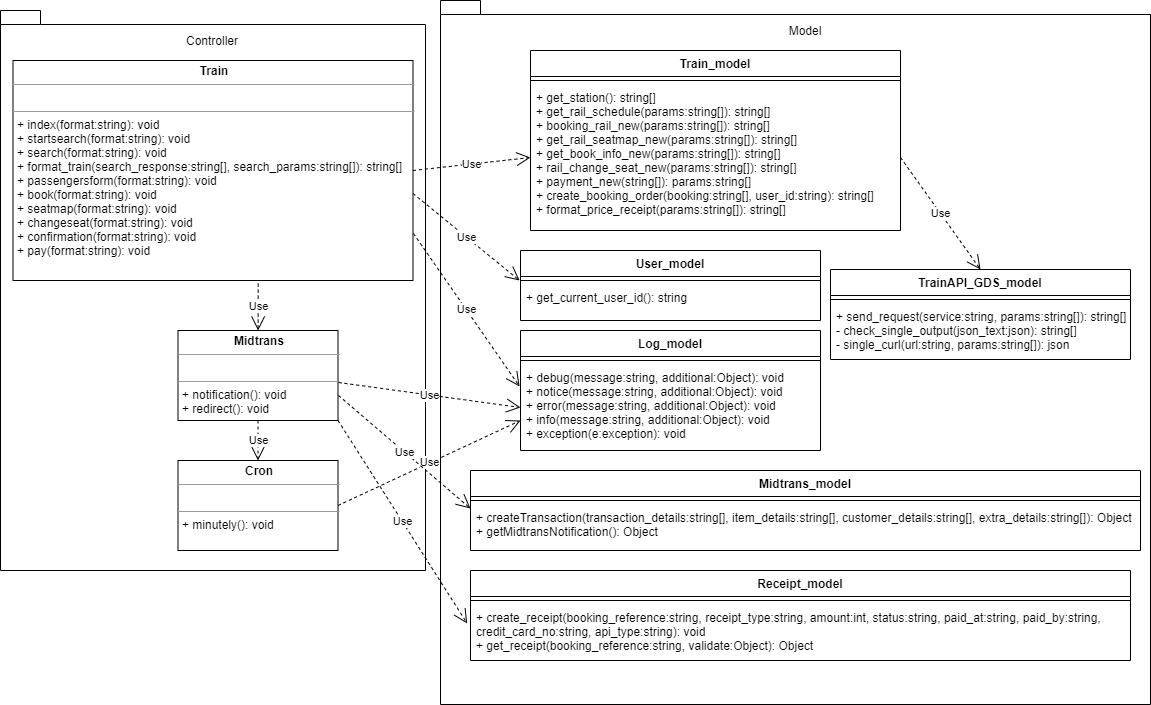
\includegraphics[width=\textwidth,height=\textheight,keepaspectratio]{Gambar/Class Diagram.png}
\caption{\textit{Class Diagram.}}
    \label{img:classdiagram}
\end{figure}

Paket \textit{Controller} berisi kumpulan \textit{controller} yang digunakan dalam proyek ini. \textit{Controller} yang digunakan antara lain:

\begin{enumerate}
    \item \textit{Train}
     \begin{itemize}
         \item index(format:string): void\\
         Metode ini merupakan metode yang pertama kali dipanggil dari \textit{controller} ini. Metode ini akan menampilkan halaman pencarian tiket. Parameter format di sini menentukan tampilan \textit{desktop} atau \textit{mobile} yang merupakan bawaan dari sistem keseluruhan. Hal ini berlaku untuk semua metode dengan parameter format.

        \item startsearch(format:string): void\\
        Metode ini akan menampilkan halaman pemilihan jadwal.
        
        \item search(format:string): void\\
        Metode ini akan memulai pencarian jadwal dan menampilkan hasil pencarian.
        
        \item format\_train(search\_response:string[], search\_params:string[]): string[]\\
        Metode ini akan memberikan format kepada parameter yang diberikan untuk dipresentasikan ke \textit{view}.
        
        \item passengersform(format:string): void\\
        Metode ini akan menampilkan halaman pengisian data pemesan dan penumpang.
        
        \item book(format:string): void\\
        Metode ini akan melakukan pemesanan untuk pengguna.
        
        \item seatmap(format:string): void\\
        Metode ini akan mendapatkan informasi tempat duduk dari kereta yang dipesan pengguna dan menampilkan halaman pemilihan kursi.
        
        \item changeseat(format:string): void\\
        Metode ini akan memberi tahu \textit{server} tentang penggantian kursi pengguna.
        
        \item confirmation(format:string): void\\
        Metode ini akan menampilkan halaman konfirmasi.
        
        \item pay(format:string): void\\
        Metode ini akan memanfaatkan \textit{model} Midtrans untuk melakukan pembayaran.
     \end{itemize}
    
    \item \textit{Midtrans}
    \begin{itemize}
        \item notification(): void\\
        Metode ini akan menangkap dan memroses notifikasi dari Midtrans.

        \item redirect(): void\\
        Metode ini akan mengarahkan pengguna sesuai kebutuhan setelah melakukan pembayaran.
    \end{itemize}
    
    \item \textit{Cron}
    \begin{itemize}
        \item minutely(): void\\
        Metode ini akan mencoba meng-\textit{issue} tiket setiap beberapa menit yang diatur sampai berhasil.
    \end{itemize}
    
\end{enumerate}

Paket \textit{Model} berisi kumpulan \textit{Model} yang dipakai dalam pembangunan proyek ini. \textit{Model} yang digunakan adalah:

\begin{enumerate}
    \item \textit{Train\_model}
    \begin{itemize}
        \item get\_station(): string[]\\
        Metode ini mendapatkan hasil modul \textit{get-station-new} dari \textit{API} GDS.
        \item get\_rail\_schedule(params:string[]): string[]\\
        Metode ini mendapatkan hasil modul \textit{get-rail-schedule-new} dari \textit{API} GDS.
        \item booking\_rail\_new(params:string[]): string[]\\
        Metode ini mendapatkan hasil modul \textit{booking-rail-new} dari \textit{API} GDS.
        \item get\_rail\_seatmap\_new(params:string[]): string[]\\
        Metode ini mendapatkan hasil modul \textit{get-rail-seatmap-new} dari \textit{API} GDS.
        \item get\_book\_info\_new(params:string[]): string[]\\
        Metode ini mendapatkan hasil modul \textit{get-book-info-new} dari \textit{API} GDS.
        \item rail\_change\_seat\_new(params:string[]): string[]\\
        Metode ini mendapatkan hasil modul \textit{rail-change-seat-new} dari \textit{API} GDS.
        \item payment\_new(string[]): params:string[]\\
        Metode ini mendapatkan hasil modul \textit{payment-new} dari \textit{API} GDS.
        \item create\_booking\_order(booking:string[], user\_id:string): string[]\\
        Metode ini membuatkan detail transaksi yang akan digunakan saat pembayaran.
        \item format\_price\_receipt(params:string[]): string[]\\
        Metode ini memberikan format untuk detail transaksi yang akan digunakan untuk pembayaran.
    \end{itemize}
    
    \item \textit{TrainAPI\_GDS\_model}
    \begin{itemize}
        \item send\_request(service:string, params:string[]): string[]\\
        Metode ini akan menjadi kerangka pemanggilan modul yang dibutuhkan dari \textit{API} GDS. Service yang menjadi parameter adalah nama modul sementara params adalah parameter yang diperlukan saat meminta hasil dari \textit{API}.
        \item check\_single\_output(json\_text:json): string[]\\
        Metode ini akan memeriksa apakah hasil dari \textit{API} berhasil atau eror. Parameter metode ini adalah kode hasil \textit{request} ke \textit{API}.
        \item single\_curl(url:string, params:string[]): json\\
        Metode ini akan melakukan \textit{request} ke \textit{API}. Metode ini dipanggil di send\_request untuk melakukan cURL.
    \end{itemize}
    
    \item \textit{User\_model}
    \begin{itemize}
        \item get\_current\_user\_id(): string\\
        Metode ini mendapatkan ID pengguna yang sedang \textit{login}. Metode ini digunakan sistem kereta api untuk fitur pengisian data penumpang secara otomatis.
    \end{itemize}
    
    \item \textit{Log\_model}
    \begin{itemize}
        \item debug(message:string, additional:Object): void\\
        Metode ini adalah metode yang dipakai untuk memberi peringatan saat terjadi sesuatu. Metode ini memiliki \textit{tag debug}.
        
        \item notice(message:string, additional:Object): void\\
        Metode ini adalah metode yang dipakai untuk memberi peringatan saat terjadi sesuatu. Metode ini memiliki \textit{tag notice}.
        
        \item error(message:string, additional:Object): void\\
        Metode ini adalah metode yang dipakai untuk memberi peringatan saat terjadi sesuatu. Metode ini memiliki \textit{tag error}.
       
        \item info(message:string, additional:Object): void\\
        Metode ini adalah metode yang dipakai untuk memberi peringatan saat terjadi sesuatu. Metode ini memiliki \textit{tag info}.
        
        \item exception(e:exception): void\\
        Metode ini adalah metode yang dipakai untuk memberi peringatan saat terjadi \textit{exception}. Metode ini mencatat \textit{exception} yang terjadi.
    \end{itemize}
    
    \item \textit{Midtrans\_model}
    \begin{itemize}
        \item createTransaction(transaction\_details:string[], item\_details:string[], customer\_details:string[], extra\_details:string[]): Object\\
        Metode ini dipakai untuk membuatkan transaksi yang digunakan untuk kebutuhan pembayaran. Parameter untuk metode ini adalah detail-detail opsional yang ingin ditambahkan transaksi.
        
        \item getMidtransNotification(): Object\\
        Metode ini meminta notifikasi dari Midtrans yang akan digunakan dalam pembayaran.
        
    \end{itemize}
    
    \item \textit{Receipt\_model}
    \begin{itemize}
        \item create\_receipt(booking\_reference:string, receipt\_type:string, amount:int, status:string, paid\_at:string, paid\_by:string, credit\_card\_no:string, api\_type:string): void\\
        Metode ini membuatkan \textit{receipt} untuk transaksi yang dibuat berdasarkan parameter yang diberikan.
        
        \item get\_receipt(booking\_reference:string, validate:Object): Object\\
        Metode ini mendapatkan \textit{receipt} transaksi yang disimpan berdasarkan parameter yang diberikan.
        
    \end{itemize}
    
\end{enumerate}

\section{Rancangan Routing}
\label{sec:rancanganrouting} 

Proyek ini dibangun menggunakan \textit{framework} CI seperti yang sudah dijelaskan di \ref{sec:codeigniter}. Dalam proyek yang menggunakan CI, \textit{URI} dapat ditentukan dalam \textit{file} \textit{routes} yang bisa ditemukan di folder \textit{config}. \textit{URI} digunakan oleh \textit{browser} untuk mengakses sebuah halaman web. \textit{File routes} memungkinkan \textit{developer} untuk memetakan \textit{URI} langsung ke fungsi \textit{controller} . Sebagai contoh, jika fungsi \textit{controller} untuk menampilkan halaman daftar kantor adalah \textit{office()}, dengan memetakan ulang \textit{URI}, \textit{developer} bisa memberikan teks daftarkantor untuk mengakses fungsi tersebut. Jadi, jika pengguna mengetik \textit{URI} example.com/daftarkantor, fungsi \textit{controller} \textit{office()} tetap terpanggil.

Proyek ini tidak memetakan ulang fungsi \textit{controller} dengan \textit{file routing}. Daftar \textit{routing} dari proyek ini dapat dilihat pada tabel \ref{tab:tabelrouting}.

\begin{table}[H]
	\centering 
	\caption{Tabel \textit{Routing}}
	\label{tab:tabelrouting}
	\begin{tabular}{|l|l|}
		\hline
		Fungsi \textit{controller} & URI\\
		\hline
		
		\hline
		index & domain.com/train\\
		\hline
		startsearch & domain.com/train/startsearch\\
		\hline
		passengersform & domain.com/train/passengersform\\
		\hline
		seatmap & domain.com/train/seatmap\\
		\hline
		confirmation & domain.com/confirmation\\
		\hline
        
	\end{tabular} 
\end{table}

\section{Screen Flow Diagram}
\label{sec:screenflowdiagram}

Rancangan alur dari halaman-halaman yang akan ada di proyek ini dapat dilihat di \ref{img:screenflowdiagram}. 

\begin{figure}[H]
\center
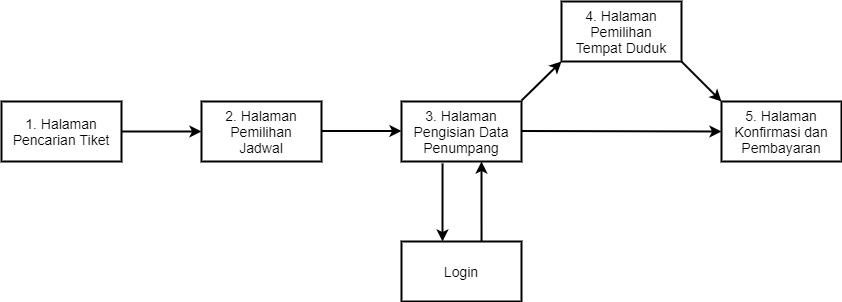
\includegraphics[width=\textwidth,height=\textheight,keepaspectratio]{Gambar/Screen Flow Diagram.png}
\caption{\textit{Screen Flow Diagram.}}
    \label{img:screenflowdiagram}
\end{figure}

\begin{enumerate}
    \item Pengguna mulai dari halaman pencarian tiket. Di sini pengguna bisa memberikan \textit{input} untuk mencari jadwal yang diinginkan.
    \item Kemudian pengguna masuk ke halaman pemilihan jadwal. Pengguna akan memilih jadwal kereta yang sudah dicari di sini.
    \item Setelah pengguna memilih jadwal, pengguna akan diminta mengisi data. Pengguna bisa masuk ke halaman \textit{login} di sini untuk menggunakan fitur yang membantu pengguna mengisi data.
    \item Pengguna bisa masuk ke halaman ini jika pengguna ingin memilih tempat duduk.
    \item Pengguna masuk ke halaman ini untuk mengkonfirmasi pesanan dan melakukan pembayaran.
\end{enumerate}  

\section{Mekanisme Pembayaran}
\label{sec:mekanismepembayaran}

Pengguna akan melakukan pembayaran setelah mengkonfirmasi kembali pesanannya. Pembayaran akan menggunakan Midtrans. Saat melakukan pembayaran, pengguna dapat memilih salah satu metode dari berbagai metode pembayaran yang ada. 

Pengguna bisa membayar menggunakan:
\begin{itemize}
    \item Kartu Kredit
    \item BCA KlikPay
    \item KlikBCA
    \item e-Pay BRI
    \item CIMB Clicks
    \item Danamon Online Banking
    \item Mandiri Clickpay
    \item ATM/Bank Transfer
    \item Indomaret
    \item LINE Pay e-cash | mandiri e-cash
    \item Pembayaran QR
    \item Akulaku
    \item Alfamart
\end{itemize}

Saat akan membayar, instruksi pembayaran untuk masing-masing jenis pembayaran dapat dilihat saat sudah memilih metode. Instruksi metode pembayaran bisa dikirim ke email pengguna jika pengguna ingin. Setelah pengguna menekan tombol bayar sekarang, pengguna tidak bisa kembali lagi untuk mengubah metode pembayaran yang diinginkan.

\subsection{Kartu Kredit}
\label{subsec:kartukredit}
Untuk melakukan pembayaran dengan kartu kredit, pengguna harus:

\begin{enumerate}
    \item Masukkan nomor kartu kredit.
    \item Masukkan waktu batas masa aktif kartu kredit.
    \item Masukkan CVV, CVV adalah 3 digit nomor keamanan yang dicetak di belakang kartu.
\end{enumerate}

\subsection{BCA KlikPay}
\label{subsec:bcaklikpay}
Untuk melakukan pembayaran dengan BCA KlikPay, pengguna harus:

\begin{enumerate}
    \item Setelah pengguna menekan tombol "Bayar Sekarang", pengguna akan diarahkan ke halaman pembayaran BCA KlikPay.
    \item Setelah Login ke Akun BCA Klikpay pengguna dengan memasukkan alamat email dan password, maka akan tampil informasi data transaksi seperti nama merchant, waktu transaksi, dan jumlah yang harus dibayar. Pilihlah jenis pembayaran KlikBCA atau BCA Card untuk transaksi tersebut.
    \item Untuk otorisasi pembayaran dengan BCA KlikPay, tekan tombol "kirim OTP", dan pengguna akan menerima kode OTP (\textit{One Time Password}) yang dikirim melalui SMS ke \textit{mobile phone} pengguna. Masukkan kode OTP tersebut pada kolom yang tersedia.
    \item Apabila kode OTP yang pengguna masukkan benar, transaksi pembayaran akan langsung diproses dan saldo rekening pengguna (untuk jenis pembayaran KlikBCA) atau limit BCA Card pengguna (untuk jenis pembayaran BCA Card) akan berkurang sejumlah nilai transaksi.
    \item Status keberhasilan transaksi pengguna akan tampil pada layar transaksi dan Anda akan menerima email notifikasi.
\end{enumerate}

\subsection{KlikBCA}
\label{subsec:klikbca}
Untuk melakukan pembayaran dengan KlikBCA, pengguna harus:

\begin{enumerate}
    \item Kunjungi situs web KlikBCA \href{https://www.klikbca.com.}{https://www.klikbca.com.})
    \item \textit{Login} menggunakan \textit{userID} KlikBCA.
    \item Pilih Menu Pembayaran \textit{e-commerce}.
    \item Pilih Kategori Lainnya.
    \item Pilih Nama Perusahaan.
    \item Klik Lanjutkan.
    \item Pilih transaksi yang ingin pengguna bayar dan pilih lanjutkan.
    \item Konfirmasikan kembali pembayaran dengan memasukkan kunci token dan pilih kirim/lanjutkan.
\end{enumerate}

\subsection{e-Pay BRI}
\label{subsec:epaybri}
Untuk melakukan pembayaran dengan e-Pay BRI, pengguna harus:

\begin{enumerate}
    \item Pastikan pengguna telah memiliki \textit{User ID} Internet Banking BRI dan sudah mendaftarkan mTOKEN sebelum melakukan pembayaran menggunakan e-Pay BRI langsung dari website BRI.
    \item Untuk mendapatkan \textit{User ID} Internet Banking BRI, silakan melakukan registrasi melalui ATM BRI terdekat.
    \item Untuk mendaftarkan mTOKEN, silakan melakukan registrasi finansial di cabang BRI terdekat.
    \item Pembayaran menggunakan e-Pay BRI akan diproses secara \textit{online}, saldo rekening BRI pengguna akan didebet secara otomatis sesuai jumlah pembelanjaan pengguna.
    \item Transaksi pengguna akan dibatalkan jika pembayaran tidak diselesaikan dalam 2 jam.
\end{enumerate}

\subsection{CIMB Clicks}
\label{subsec:cimbclicks}
Untuk melakukan pembayaran dengan CIMB Clicks, pengguna harus:

\begin{enumerate}
    \item Pastikan pengguna telah memiiki \textit{User ID} CIMB Clicks dan sudah mendaftarkan mPIN sebelum melakukan pembayaran melalui CIMB Clicks ini.
    \item Pembayaran melalui CIMB Clicks akan diproses secara online, saldo rekening CIMB pengguna akan didebet secara otomatis sesuai jumlah pembelanjaan.
    \item Transaksi pengguna akan dibatalkan jika pembayaran tidak diselesaikan dalam 2 jam.
\end{enumerate}

\subsection{Danamon Online Banking}
\label{subsec:danamononlinebanking}
Untuk melakukan pembayaran dengan Danamon Online Banking, pengguna harus:

\begin{enumerate}
    \item Masukkan \textit{User ID} dan \textit{Password} Danamon Online Banking pengguna dan pilih sumber rekening untuk pembayaran.
    \item Cek rincian informasi transaksi, masukkan Kode Token, lalu tekan lanjut.
    \item Konfirmasi transaksi pembayaran akan muncul, pembayaran selesai. Simpan informasi referensi \textit{merchant} dan referensi pembayaran, tekan Lanjut untuk kembali ke situs \textit{merchant}.
\end{enumerate}

\subsection{Mandiri Clickpay}
\label{subsec:mandiriclickpay}
Untuk melakukan pembayaran dengan Mandiri Clickpay, pengguna harus:

\begin{enumerate}
    \item Aktifkan Mandiri token dengan menekan tombol <.
    \item Masukkan password Mandiri token.
    \item Tekan 3 ketika Mandiri token menampilkan APPLI.
    \item Masukkan Input 1 dan tekan < selama 3 detik.
    \item Masukkan Input 2 dan tekan < selama 3 detik.
    \item Masukkan Input 3 dan tekan < selama 3 detik.
    \item Masukkan kode yang dihasilkan Mandiri token ke kolom Masukkan challenge token.
\end{enumerate}

\subsection{ATM/Bank Transfer}
\label{subsec:atmtransfer}
Untuk melakukan pembayaran dengan ATM/Bank Transfer, pengguna harus:

\begin{enumerate}
    \item Pada menu utama, pilih Transaksi Lainnya.
    \item Pilih Transfer.
    \item Pilih Rek Bank Lain.
    \item Masukkan nomor 009 (kode Bank BNI) lalu tekan Benar.
    \item Masukkan jumlah tagihan yang akan dibayar secara lengkap, pembayaran dengan jumlah tidak sesuai akan otomatis ditolak.
    \item Masukkan 16 digit No. Rekening pembayaran lalu tekan Benar.
    \item Pada halaman konfirmasi transfer akan muncul jumlah yang dibayarkan, nomor rekening \& nama \textit{Merchant}. Jika informasi telah sesuai tekan Benar.
\end{enumerate}

Instruksi di atas adalah jika pengguna memilih pilihan bank lain setelah memilih metode transfer. Pilihan selain bank lain adalah BCA, Permata, Mandiri dan BNI. Untuk masing-masing bank, ada sedikit penyesuaian tapi pada dasarnya semua mengikuti alur yang sama.

\subsection{Indomaret}
\label{subsec:indomaret}
Untuk melakukan pembayaran lewat Indomaret, pengguna harus:

\begin{enumerate}
    \item Setelah melakukan konfirmasi pembayaran, pengguna akan diberikan Kode Pembayaran yang unik.
    \item Salinlah kode pembayaran dan jumlah pembayaran yang akan dibayarkan. Midtrans juga akan mengirimkan salinan Kode Pembayaran dan instruksi pembayaran melalui email.
    \item Pergi ke toko Indomaret terdekat dan berikanlah nomor kode pembayaran ke kasir.
    \item Kasir Indomaret akan mengkonfirmasi transaksi dengan menanyakan jumlah pembayaran dan nama \textit{merchant}.
    \item Konfirmasikan pembayaran ke kasir.
    \item Pengguna akan mendapatkan email konfirmasi pembayaran
    \item Simpan struk transaksi.
\end{enumerate}

\subsection{LINE Pay e-cash | mandiri e-cash}
\label{subsec:linepayecash}
Untuk melakukan pembayaran dengan LINE Pay e-cash | mandiri e-cash, pengguna harus:

\begin{enumerate}
    \item Pastikan pengguna telah mendaftarkan nomor ponsel untuk LINE Pay e-cash | mandiri e-cash.
    \item Klik Bayar Sekarang.
    \item Masukkan nomor ponsel yang sudah terdaftar dan PIN.
    \item Tunggu kiriman SMS e-cash yang berisi \textit{One Time Password} (OTP).
    \item Masukkan kode 6 angka OTP yang diterima, kemudian tekan tombol bayar untuk melakukan pembayaran.
    \item Jika SMS OTP belum diterima / kadaluarsa dalam 5 menit. Klik tombol batal untuk mengulang transaksi.

\end{enumerate}

\subsection{Pembayaran QR}
\label{subsec:pembayaranqr}
Untuk melakukan pembayaran dengan pembayaran QR, pengguna harus:

\begin{enumerate}
    \item Buka aplikasi pembayaran pilihan. Pastikan aplikasi sudah mendukung layanan QRIS.
    \item Pindai kode QR yang ada pada monitor.
    \item Periksa detail transaksi pada aplikasi, lalu tap tombol Bayar.
\end{enumerate}

\subsection{Akulaku}
\label{subsec:akulaku}
Akulaku adalah aplikasi yang memudahkan Anda berbelanja secara kredit tanpa kartu kredit. Untuk melakukan pembayaran dengan Akulaku, pengguna harus:

\begin{enumerate}
    \item Tekan tombol "Bayar Sekarang", lalu pengguna akan diarahkan ke halaman Pusat Pembayaran Akulaku.
    \item Pilih tenor cicilan yang diinginkan, lalu Login ke akun Akulaku dengan memasukkan nomor telepon \textit{mobile} dan password.
    \item Masukkan kode verifikasi (OTP) yang telah dikirimkan ke ponsel pengguna, lalu klik tombol "Selanjutnya"
    \item Akan tampil halaman konfirmasi, lalu pengguna dapat menyelesaikan transaksi.
\end{enumerate}

\subsection{Alfamart}
\label{subsec:alfamart}
Untuk melakukan pembayaran lewat Alfamart, pengguna harus:

\begin{enumerate}
    \item Setelah melakukan konfirmasi pembayaran, pengguna akan diberikan Kode Pembayaran yang unik.
    \item Salinlah kode pembayaran dan jumlah pembayaran yang akan dibayarkan. Midtrans akan mengirimkan salinan kode pembayaran dan instruksi pembayaran melalui email.
    \item Silakan pergi ke gerai Alfamart, Alfamidi, atau Dan+Dan terdekat dan berikanlah nomor kode pembayaran ke kasir.
    \item Kasir akan mengkonfirmasi transaksi dengan menanyakan jumlah transaksi dan nama \textit{merchant}.
    \item Konfirmasikan pembayaran ke kasir.
    \item Pengguna akan mendapatkan email konfirmasi pembayaran.
    \item Simpan struk transaksi.
\end{enumerate}

\section{Perancangan Sistem}
\label{sec:perancangansistem}
Sistem pemesanan tiket kereta yang akan dibuat akan memiliki beberapa fitur dan halaman yang mirip dengan sistem pemesanan tiket pesawat. Fitur-fitur yang mirip dan pertimbangannya akan dijelaskan di \ref{sec:perancanganhalaman} dan lebih detail di \ref{chap:implementasi}. Antarmuka dibuat mirip demi menjaga konsistensi tampilan yang sudah ada dan memudahkan mendaur ulang tampilan-tampilan yang pernah dibuat. Perbedaan paling mencolok dari penerbangan dan kereta adalah adanya tambahan tampilan pemilihan kursi untuk kereta yang tidak dimiliki penerbangan.

Halaman-halaman yang akan dibuat akan mengimplementasikan respon-respon dari \textit{GDS API}. \textit{API} akan menangani \textit{booking}, \textit{cancel} dan mencari jadwal. Sistem yang dibuat akan mengambil respon dari \textit{API} dan menampilkannya untuk pengguna. Masing-masing halaman akan mengimplementasikan modul-modul \textit{API} yang ada. Penjelasan lebih mendalam dapat dilihat di \ref{chap:implementasi}.

Secara garis besar, halaman-halaman yang dibuat akan meminta sebuah informasi atau menyampaikan informasi pada \textit{API}. Data yang diterima atau dikirimkan akan diformat sehingga mudah dilihat oleh pengguna dan diterima oleh \textit{API}. Selain \textit{GDS API}, sistem juga mengirim dan menerima data dari Midtrans untuk memberikan konfirmasi pembayaran. Respon dari Midtrans juga akan dikirimkan oleh sistem kepada \textit{GDS API} untuk mengkonfirmasi \textit{booking} yang sudah dibayar.

\section{Perancangan Antarmuka dan Fitur}
\label{sec:perancanganhalaman} 

Situs kereta api pada umumnya mencakup 5 halaman utama. Halaman yang dimaksud adalah halaman untuk mencari tiket, memilih jadwal kereta, mengisi data pemesan dan penumpang, memilih tempat duduk dan yang terakhir adalah untuk konfirmasi dan pembayaran. Halaman pencarian tiket akan menjadi halaman pertama yang dilihat pengguna saat ingin melakukan pemesanan. Kemudian pengguna akan masuk ke halaman untuk memilih jadwal. Setelah memilih jadwal, pengguna akan diminta mengisi data pemesan dan data penumpang. Pada halaman ini, saat pengguna sudah mengisi semua data yang diperlukan, pengguna diberi pilihan untuk langsung ke halaman mengubah kursi atau konfirmasi. Halaman konfirmasi adalah halaman terakhir dan juga merupakan halaman untuk melakukan pembayaran.

Desain dari situs kereta api ini akan mengikuti desain dari 2 fitur lainnya yaitu hotel dan penerbangan untuk menjaga konsistensi. Pada dasarnya, alur pemesanan tiket kereta mirip dengan alur pemesanan tiket penerbangan sehingga desain yang sama bisa digunakan. Penyesuaian perlu dilakukan di beberapa tempat dan akan dilakukan saat membangun web. Perbedaan paling besar dari fitur penerbangan yang sudah ada dan kereta yang akan dibuat adalah adanya halaman untuk memilih kursi.

\subsection{Halaman Pencarian Tiket}
\label{subsec:rancanganpencariantiket}

Halaman pencarian tiket adalah halaman pertama yang akan dijumpai pengguna. Halaman ini akan memberikan masukan untuk mencari jadwal yang diinginkan. Halaman ini memiliki masukan berupa asal, tujuan, tanggal keberangkatan, tanggal pulang yang bersifat opsional dan pilihan kelas (ekonomi, bisnis, eksekutif dan lain-lain) seperti pada gambar \ref{img:rancangancaritiket}. Setelah memasukkan data yang diperlukan, tekan tombol pencarian untuk mencari jadwal sesuai masukan yang diberikan.

\begin{figure}[H]
\center
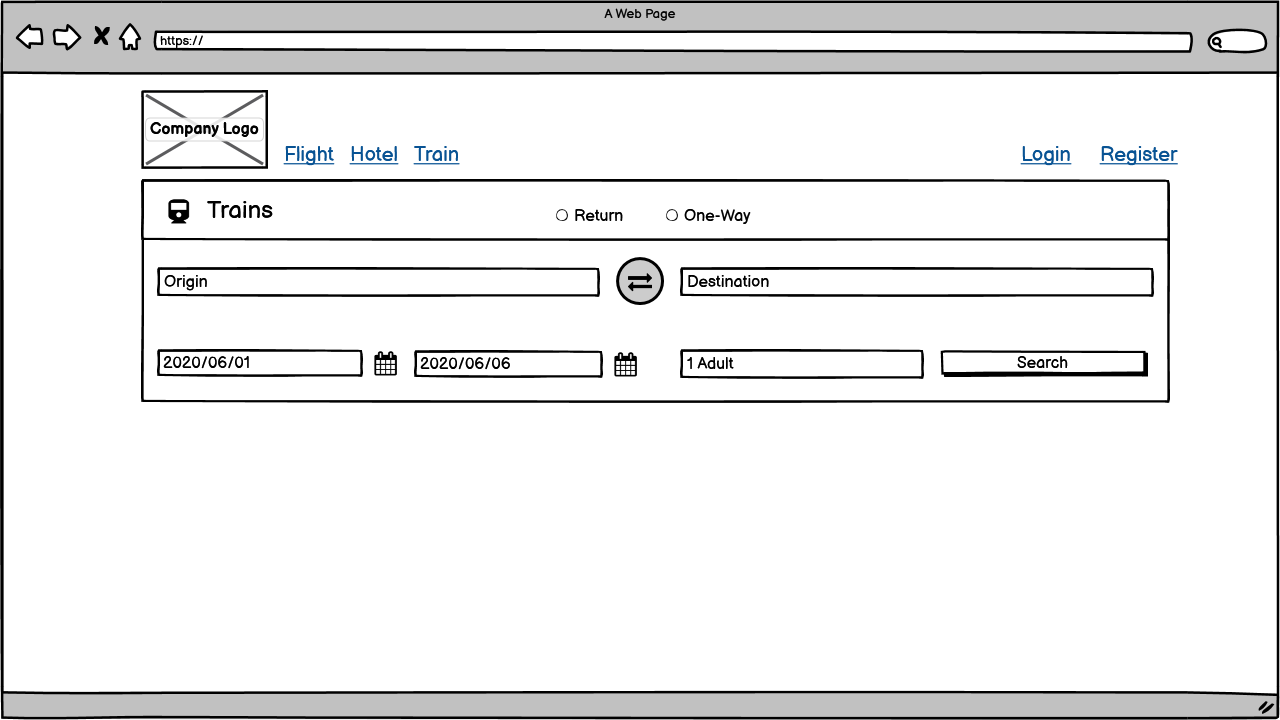
\includegraphics[width=\textwidth,height=\textheight,keepaspectratio]{Gambar/Halaman Pencarian Tiket.png}
\caption{Rancangan Halaman Pencarian Tiket.}
    \label{img:rancangancaritiket}
\end{figure}

Dalam perancangan proyek ini, desain yang diambil dari bagian penerbangan perlu disesuaikan dengan tempat pemesanan tiket \textit{online} dari situs lain. Setelah membandingkan dengan beberapa situs lainnya, masukan pilihan kelas pada umumnya tidak ditemukan di tempat lain. Ini dikarenakan pemilihan kelas langsung dilakukan saat memilih jadwal kereta. Dari daftar jadwal yang ditampilkan, pengguna bisa melihat kelas dan sub-kelas tiap pilihan saat ingin memilih.

Halaman pencarian tiket memiliki fitur \textit{auto-complete} untuk membantu pengguna memilih tempat asal dan tujuan. Saat pengguna mengetik stasiun asal atau tujuan, sistem akan memberikan \textit{auto-complete} untuk mempermudah pengguna memilih stasiun. Tujuan lain dari fitur ini adalah mencegah pengguna memasukkan nama stasiun yang salah sehingga pencarian gagal. \textit{Auto-complete} bisa muncul dari mengetik nama stasiun langsung atau mengetik kode stasiun.

Selain fitur \textit{auto-complete}, memilih tanggal juga harus diatur sehingga pengguna tidak bisa memilih tanggal mustahil. Contoh tanggal mustahil adalah mencari tiket berangkat dari tanggal sebelum tanggal saat itu atau membeli tiket pulang dengan tanggal yang lebih awal dibanding tiket berangkat. Kedua hal itu hanya akan menghasilkan pencarian yang kosong. Tanggal juga diatur 1 minggu dari tanggal saat itu mengikuti fitur penerbangan. Jika pengguna memilih perjalanan pulang pergi, tanggal pulang dipilihkan 1 minggu dari tanggal keberangkatan mengikuti fitur penerbangan.

Fitur terakhir dari halaman ini yang akan dibuat saat implementasi nanti adalah mengatur jumlah penumpang sesuai dengan aturan KAI. Setidaknya harus ada 1 penumpang dewasa saat memesan. Sekali memesan, penumpang hanya boleh ada 4 orang termasuk bayi. Jumlah bayi tidak boleh melebihi jumlah dewasa.

\subsection{Halaman Pemilihan Jadwal Kereta Api}
\label{subsec:rancanganpemilihanjadwal}

Halaman berikutnya adalah halaman memilih jadwal. Halaman ini menampilkan jadwal sesuai dengan masukan yang diberikan di halaman sebelumnya. Jadwal yang ditampilkan akan memuat informasi yang penting saat memilih seperti tanggal berangkat, harga, nama kereta, kelas beserta sub-kelas dan jumlah sisa kursi seperti pada gambar \ref{img:rancanganjadwalberangkat}. Terdapat juga beragam filter di kiri layar untuk memudahkan pengguna memilih jadwal yang dia inginkan.

\begin{figure}[H]
\center
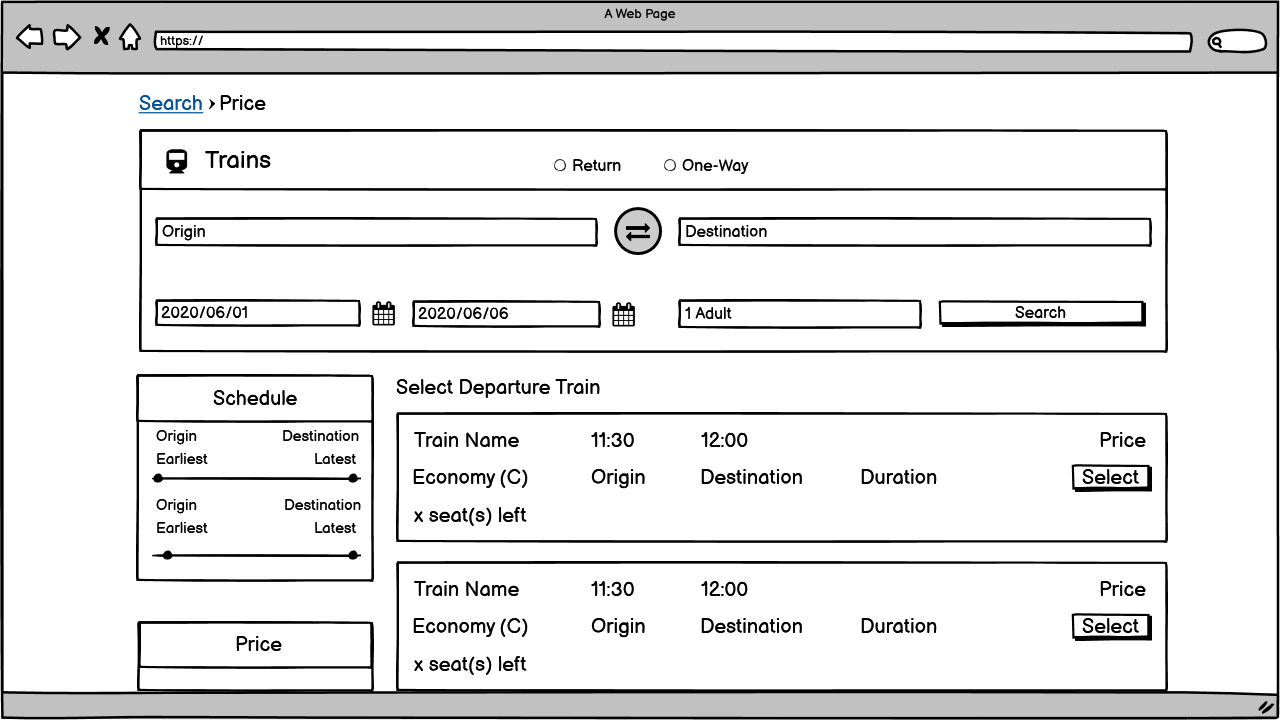
\includegraphics[width=\textwidth,height=\textheight,keepaspectratio]{Gambar/Halaman Pemilihan Jadwal (Berangkat).png}
\caption{Rancangan Halaman Pemilihan Jadwal Keberangkatan.}
    \label{img:rancanganjadwalberangkat}
\end{figure}

Fitur pertama dari halaman ini adalah menampilkan jadwal sesuai dengan masukan yang diberikan pengguna di halaman sebelumnya. Informasi yang ditampilkan per jadwal adalah nama dan nomor kereta, kelas dan sub-kelas kereta, ketersediaan kursi, stasiun awal dan tujuan, lamanya waktu perjalanan dan harga. Filter akan mengikuti informasi jadwal yang ditampilkan. Jika pengguna memilih perjalanan pulang pergi maka jadwal pulang akan disembunyikan dan baru akan ditampilkan saat pengguna sudah memilih jadwal berangkat seperti pada gambar \ref{img:rancanganjadwalpulang}.

Fitur lain dari halaman pemilihan jadwal adalah adanya tempat pencarian tiket yang sama seperti halaman sebelumnya di atas hasil pencarian. Adanya akses untuk langsung mencari kembali jadwal lain di sini memudahkan pengguna dalam kasus mereka ingin mengganti atau salah memasukkan data. Selain itu, hal ini memudahkan pengguna untuk mencari jadwal lain jika pengguna tidak mendapatkan hasil dari pencarian sebelumnya karena pengguna tidak perlu kembali ke halaman pertama. Data yang dimasukkan di halaman pertama ditampilkan kembali di halaman ini agar pengguna bisa memeriksa juga masukan dia di halaman pertama tidak salah jika hasil pencariannya kosong.

\begin{figure}[H]
\center
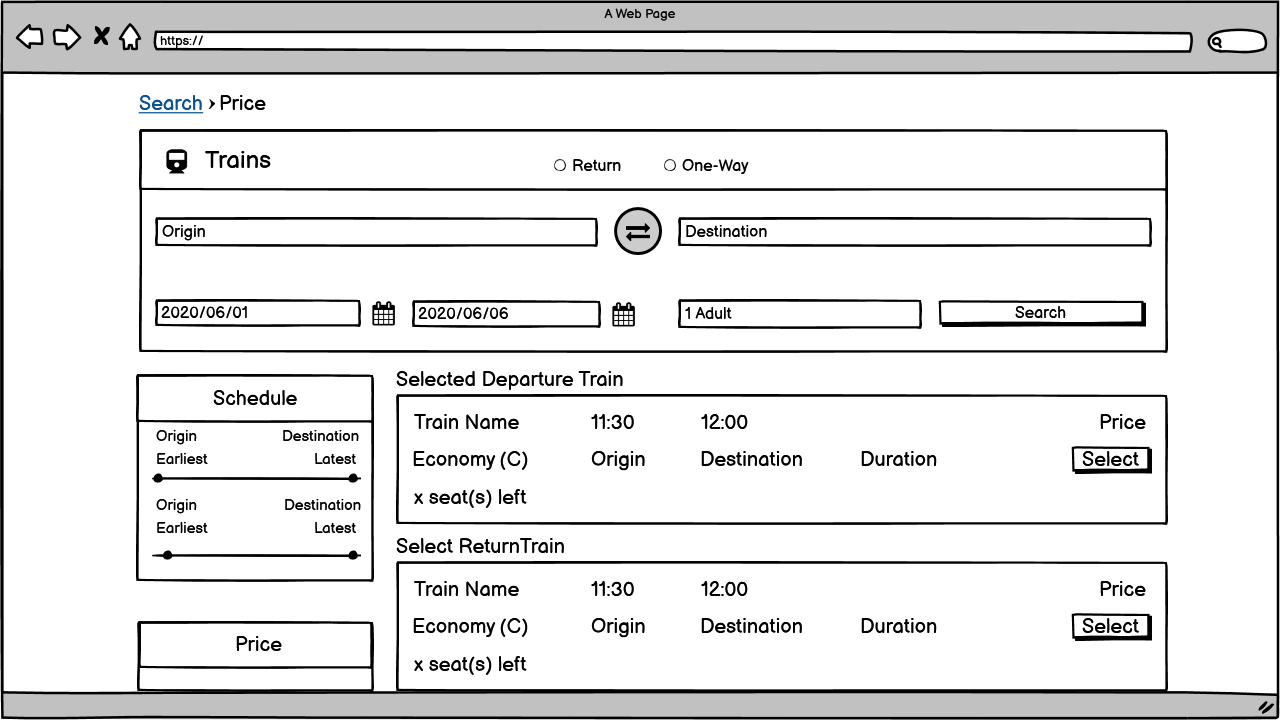
\includegraphics[width=\textwidth,height=\textheight,keepaspectratio]{Gambar/Halaman Pemilihan Jadwal (Kepulangan).png}
\caption{Rancangan Halaman Pemilihan Jadwal Kepulangan.}
    \label{img:rancanganjadwalpulang}
\end{figure}

Untuk mempermudah pencarian jadwal yang diinginkan, halaman ini memiliki fitur filter yang menggunakan beberapa faktor. Filter dapat dilakukan berdasarkan waktu, harga dan nama kereta. Fitur filter mengikuti jadwal-jadwal yang ditampilkan. \textit{Slider} waktu akan menyesuaikan dengan jadwal keberangkatan paling awal untuk kiri dan paling akhir untuk kanan. \textit{Slider} harga menggunakan harga paling murah untuk kiri dan paling mahal untuk kanan. Filter untuk memilih nama kereta dibuat dengan menggunakan \textit{checkbox}. Nama kereta yang tidak diceklis tidak akan ditampilkan di hasil pencarian. Data filter tersebut akan berganti mengikuti apakah yang ditampilkan adalah jadwal berangkat atau jadwal pulang seperti pada gambar \ref{img:rancanganjadwalpulang}.

Jika pengguna memilih perjalanan 2 arah, setelah pengguna memilih kereta keberangkatan, jadwal berangkat disembunyikan dan jadwal kereta pulang ditampilkan. Jadwal yang dipilih tetap ditampilkan di atas jadwal pulang seperti pada gambar \ref{img:rancangankonfirmasijadwal}. Data yang dipakai di filter berubah seperti yang sudah disebutkan di paragraf sebelumnya. Setelah pengguna memilih jadwal, \textit{pop-up} konfirmasi yang berisi jadwal yang dipilih dan harga akan muncul. \textit{Cancel}, \textit{close} dan menekan di luar kotak akan dianggap respon yang sama yaitu batal. \textit{Next} akan membawa pengguna ke halaman selanjutnya. 

\begin{figure}[H]
\center
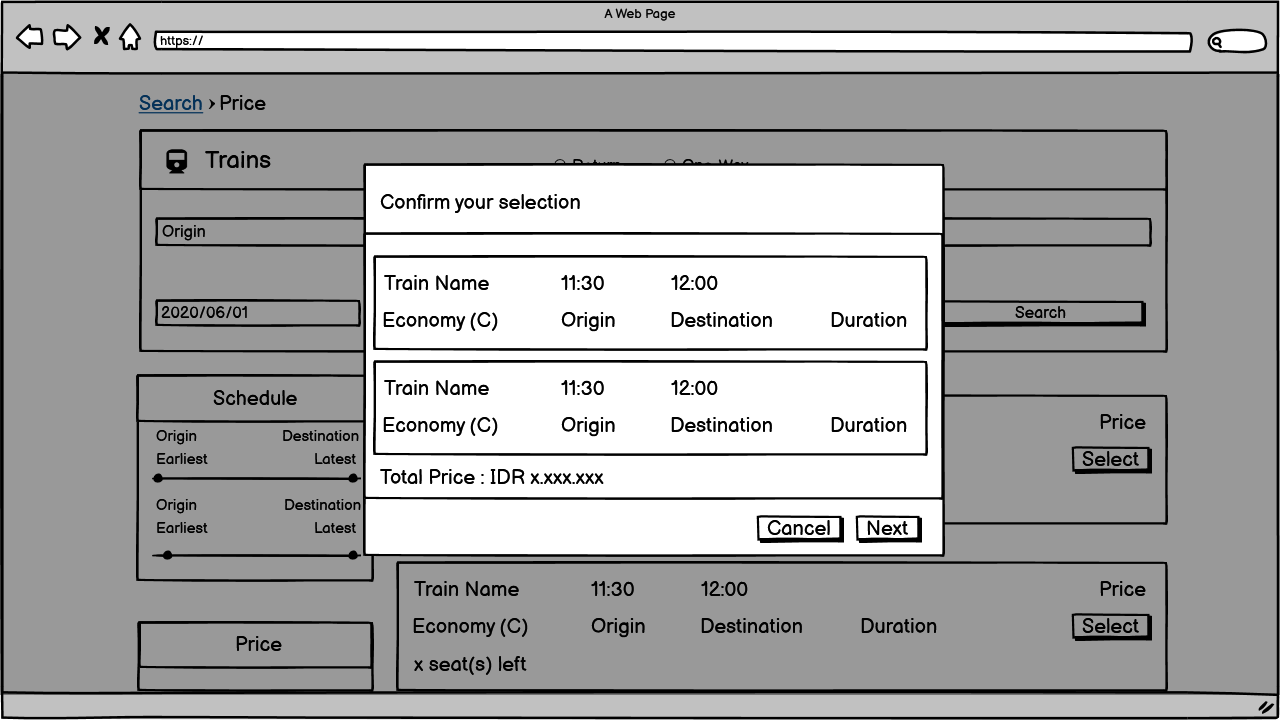
\includegraphics[width=\textwidth,height=\textheight,keepaspectratio]{Gambar/Halaman Pemilihan Jadwal (Konfirmasi).png}
\caption{Rancangan Halaman Konfirmasi Pemilihan Jadwal.}
    \label{img:rancangankonfirmasijadwal}
\end{figure}

\subsection{Halaman Pengisian Data Penumpang}
\label{subsec:rancanganpengisiandata}

Halaman ketiga adalah halaman pengisian data penumpang. Halaman ini akan menampilkan \textit{form} yang harus diisi oleh pengguna untuk memesan. Di samping \textit{form}, tersedia rangkuman jadwal yang sudah dipilih oleh pengguna dari halaman sebelumnya. Berbeda dengan pesawat seperti yang ditampilkan di gambar \ref{img:rancanganisidata}, pengguna harus mengisi 2 jenis \textit{form} yaitu data pemesan dan data penumpang. Data pemesan yang dibutuhkan adalah \textit{title (Mr., Mrs., Ms.)}, nama dan telepon dengan email sebagai pilihan opsional. Data penumpang yang diminta hanya berupa nama dan identitas (nomor KTP/KK). Selain itu, ada juga opsi untuk masuk ke halaman pemilihan kursi yang menjadi perbedaan paling besar antara bagian pemesanan pesawat dan kereta dalam proyek ini.

Fitur halaman ini adalah pengecekan data sudah dimasukkan atau belum. Jika pengguna mencoba menekan tombol \textit{next} tanpa memasukkan data yang dibutuhkan, maka pengguna akan diminta mengisi datanya terlebih dahulu. Selain itu sama seperti \ref{subsec:rancanganpemilihanjadwal}, saat pengguna sudah selesai mengisi data, muncul \textit{pop-up} konfirmasi yang meminta pengguna untuk mengecek kembali data yang dimasukkan.

\textit{Sidebar} memuat informasi-informasi penting pemesanan. Data yang ditampilkan paling atas adalah tanggal keberangkatan. Tepat di bawahnya terdapat informasi nama dan nomor kereta, jam dan stasiun keberangkatan serta jam dan stasiun tujuan untuk keberangkatan dan pulang. Dilanjutkan dengan jumlah penumpang dewasa dan bayi yang berguna juga untuk menyamakan dengan jumlah data dan tipe penumpang yang harus diisi. Terakhir di paling bawah, terdapat harga total dari jadwal yang dipilih.

\begin{figure}[H]
\center
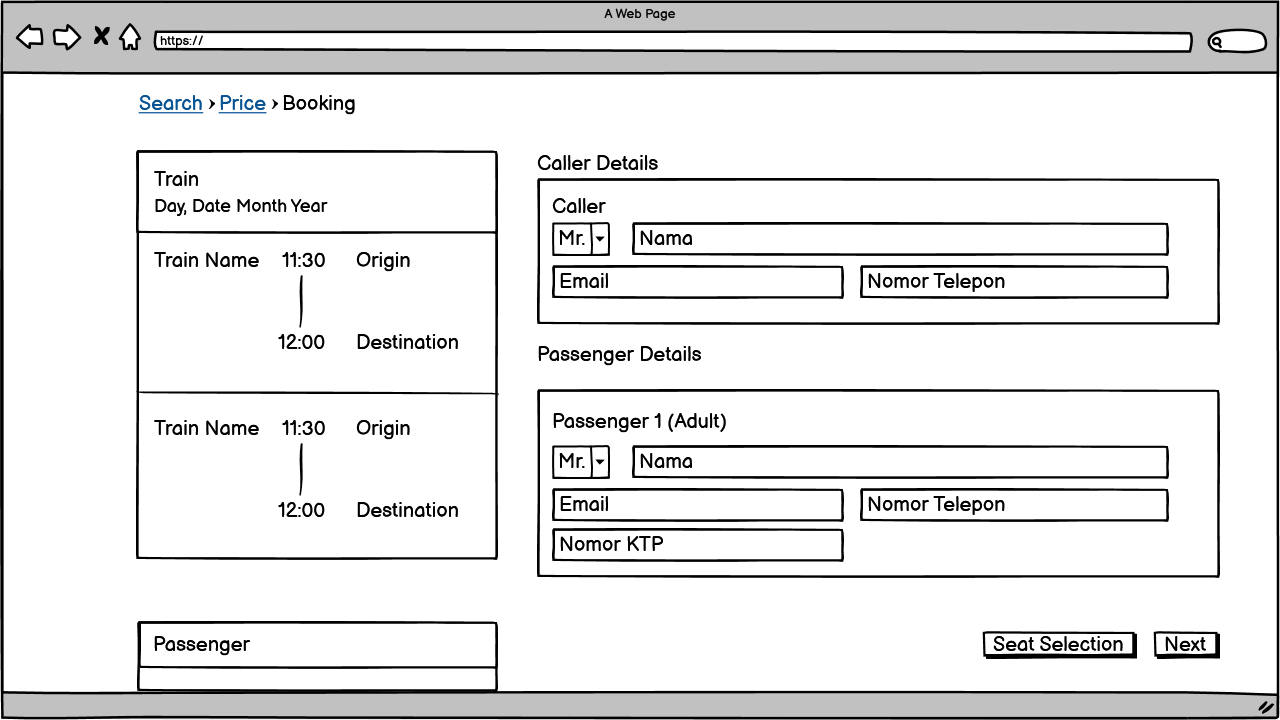
\includegraphics[width=\textwidth,height=\textheight,keepaspectratio]{Gambar/Halaman Pengisian Identitas.png}
\caption{Rancangan Halaman Pengisian Data Penumpang.}
    \label{img:rancanganisidata}
\end{figure}

Di halaman ini tersedia fitur untuk \textit{login} jika pengguna sudah terdaftar. Dengan melakukan \textit{login} pengguna, pengguna dapat menggunakan fitur \textit{fill from address book}. Fitur ini akan mengisikan data yang dibutuhkan secara otomatis jika dipilih dari \textit{dropdown} yang tersedia.

\subsection{Halaman Pemilihan Tempat Duduk}
\label{subsec:rancanganpemilihankursi}

Halaman keempat yang bersifat opsional dalam pemesanan tiket kereta api adalah pemilihan tempat duduk. Pengguna masuk ke halaman ini jika mereka ingin mengganti kursi yang dipesan. Halaman ini menampilkan representasi pemetaan kursi dari kereta yang dapat dilihat di gambar \ref{img:rancanganpilihkursi}. Pengguna bisa memilih kursi yang mereka inginkan dengan mengklik langsung di kotak-kotak yang melambangkan kursi.

Pengguna dapat memilih kursi dengan memilih kotak sesuai dengan penjelasan masing-masing kotak di bawah peta tempat duduk. Selain itu, pengguna bisa memilih gerbong yang dia ingin dengan menekan \textit{dropdown} di bawah informasi penumpang. Tombol \textit{restore default} ada untuk mengembalikan pilihan ke semula jika pengguna salah memilih tempat. Pengguna dapat memilih kursi sesuai dengan jumlah penumpang dewasa yang ada.

Setelah pengguna memilih kursi untuk keberangkatan dan kepulangan, pengguna menekan tombol \textit{next}. Sama seperti halaman-halaman sebelumnya, \textit{pop-up} konfirmasi akan muncul agar pengguna bisa memastikan pilihannya sudah benar. Setelah memastikan pilihannya sudah benar, pengguna masuk ke halaman selanjutnya.

\begin{figure}[H]
\center
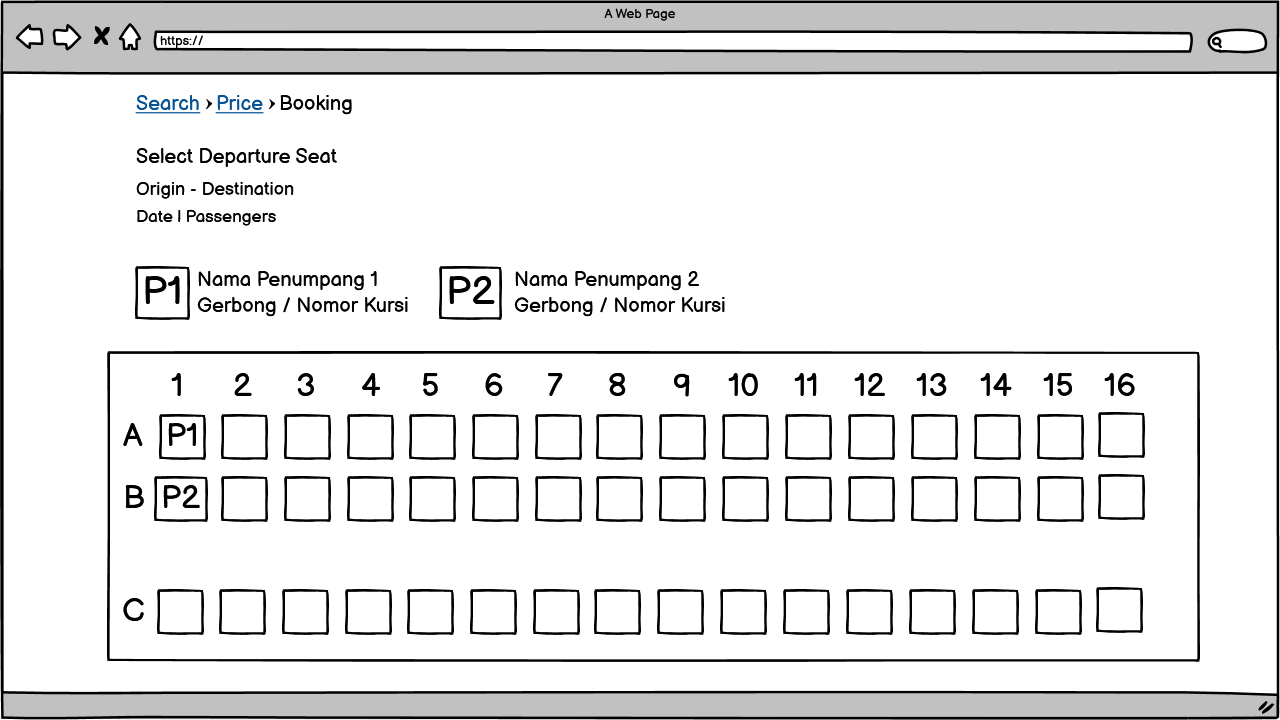
\includegraphics[width=\textwidth,height=\textheight,keepaspectratio]{Gambar/Halaman Pemilihan Tempat Duduk.png}
\caption{Rancangan Halaman Pemilihan Tempat Duduk.}
    \label{img:rancanganpilihkursi}
\end{figure}

\subsection{Halaman Konfirmasi dan Pembayaran}
\label{subsec:rancangankonfirmasi}

Halaman terakhir adalah halaman konfirmasi dan pembayaran. Di halaman terakhir ini, informasi-informasi penting yang terkait dengan pemesanan ditampilkan lagi agar bisa dicek ulang oleh pengguna seperti pada gambar \ref{img:rancangankonfirmasi}. \textit{Sidebar} yang ditampilkan di \ref{subsec:rancanganpengisiandata} digunakan lagi di sini untuk memberi informasi jadwal yang dipilih. Fitur voucher akan dihilangkan sementara untuk membuat bagian ini lebih sederhana.

Saat pengguna ingin melakukan pembayaran, maka halaman akan dialihkan ke Midtrans seperti yang sudah dijelaskan di \ref{sec:midtransapi}. Pengguna melakukan verifikasi sekali lagi pesanannya baru melakukan pembayaran. Setelah melakukan pembayaran, pengguna akan kembali ke halaman akhir dan transaksi selesai.

\begin{figure}[H]
\center
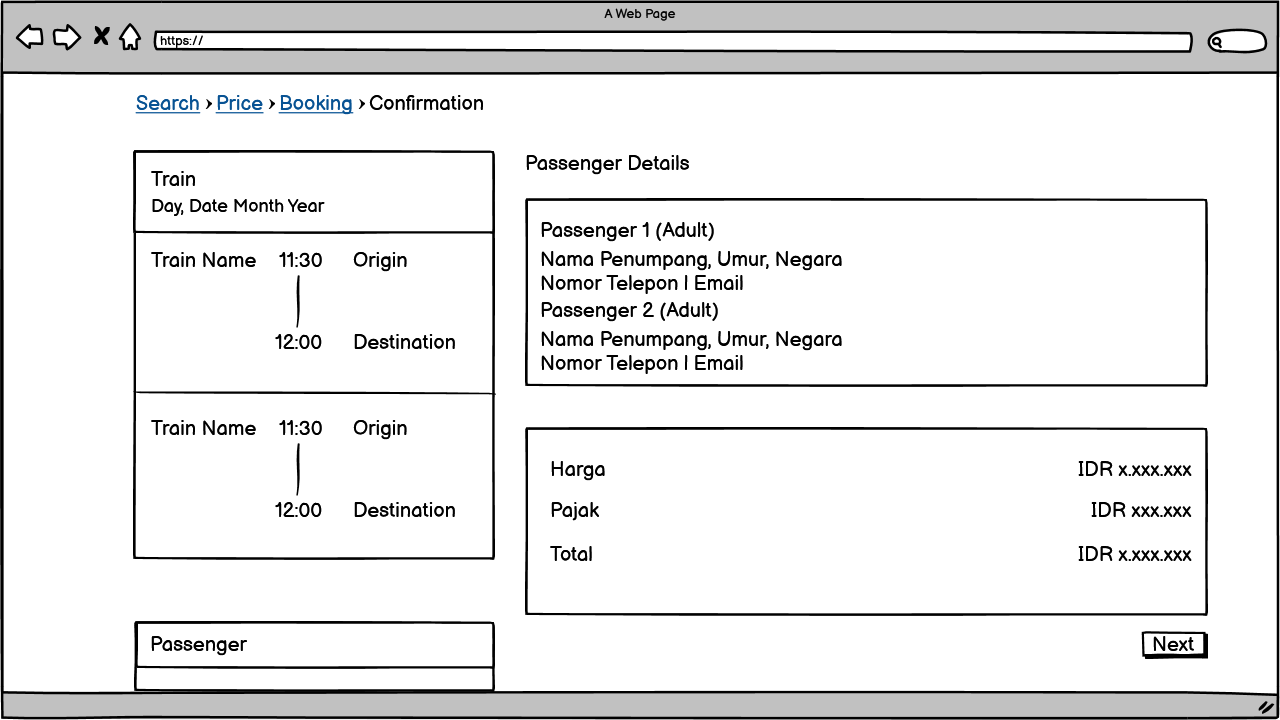
\includegraphics[width=\textwidth,height=\textheight,keepaspectratio]{Gambar/Halaman Konfirmasi.png}
\caption{Rancangan Halaman Konfirmasi.}
    \label{img:rancangankonfirmasi}
\end{figure}
